Begriffe:
\begin{description}
http://cgm.cs.mcgill.ca/~mcleish/644/Projects/DerekJohns/Sweep.htm

\item[site] ist ein Punkt in der Ebene.
\item[beach line] teilt die Ebene in zwei Bereiche. Oberhalb der beach line sind alle Bereiche die potentiell zu den Voronoi Regionen der jeweiligen Punkte gehören werden. Unterhalb der beach line alle Punkte Punkte zu denen noch keine Aussage getroffen werden kann. Die Punkte auf der beach line sind equidistant zum zugehörigen Punkt und zur sweep line.
\item[breakpoint] sind die Schnittpunkte der Parabeln.
\item[site Event] tritt auf, wenn die Sweepline einen Punkt ("`site"') trifft.
\item[circle Event] tritt auf, wenn Kreisbögen verschwinden.
\end{description}

Datenstruktur:
\begin{description}
\item[sweep line status (SLS)] ...
\item[event point schedule (EPS)] ...

\item[priority queue] enthält site events und circle events. Die Priorität ist durch die $X$-Koordinate gegeben, d.h. tritt das Event weiter links auf, so ist die Priorität höher. Initialisiert wird die priority queue mit allen zu Beginn gegebenen Punkten.
\item[edge vertex list] speichert das entstehende Voronio Diagramm. Durch ein site event entsteht eine neue Voronoi Kante. Durch ein circle event (zwei oder mehr treffen sich) entsteht ein Voronoi Knoten und zusätzlich eine Kante die an diesem Knoten beginnt.
\item[balanced binary search tree] erhält die Topologie der beach line. So richtig einfach ist das nicht mit dem Baum, verstehe nicht wie ein Knoten 3 Blätter haben kann, wenn es doch ein Binärbaum ist.
\end{description}

INIT:\\
EPS: $p_1={0,0}$, $p_2={1,2}$, $p_3={2,3}$, $p_4={4,3}$\\
beachline: $\emptyset$\\
VD: $\emptyset$\\

EVENT1: $p_1$ - site event\\
EPS: $p_2={1,2}$, $p_3={2,3}$, $p_4={4,3}$\\
beachline: $p_1$ mit Parabel (keine Breakpoints yet) wird Wurzel (hm, malen oder so)\\
VD: $\emptyset$\\

EVENT2: $p_2={1,2}$ - site event\\
EPS: $p_3={2,3}$, $p_4={4,3}$\\
beachline: bild mit binärbaum, irgendwie verstehe ich nicht warum es Knoten mit 3 leaves gibt, drei Parabelstücke, wie auch immer die heißen werden, mal schauenw as das Wörterbuch sagt\\
VD: eine Kante, bzw. naja so richtig ist es ja noch keine Kante, gibt ja noch keine zwei breakpoints wo sich ne Kante malen lassen würde\\
kommt kein Kreisevent dazu\\

EVENT3: $p_3={2,3}$ - site event




Super, wenn Du das machst. Ich habe mal nur die Bilder produziert. Einige interne Anmerkungen:
\begin{itemize}
\item Im Code läuft die Sweep-Line von oben nach unten, weil es so einfacher ist mit Parabeln zu rechnen. In der Vorlesung wurde die Sweep-Line von links nach rechts gezogen, weswegen ich beim Produzieren der Bilder die Punkte um $45^\circ$ gedreht, den Algo angewendet, zurückgedreht habe. Wir wollen ja die Aufgabe so lösen, wie sie auch gedacht ist :) Zusätzlich habe ich absolut verschoben und - für bessere Bilder - etwas nach oben skaliert
\item Solltest Du in den Code gucken: Ich benutze als Datenstruktur für die Beachline derzeit nur eine Liste anstatt eines Suchbaumes (ich ändere das noch bei Gelegenheit), weil das einfacher zu implementieren war. Auf die Bilder hat das keine Auswirkung, es ist aber wichtig zu verstehen das man nur bei Verwendung einer $\log n$-Such-Datenstruktur eine Laufzeit von $O(n\cdot\log n)$ erreichen kann.
\item Für jeden Schritt muss m.E. erklärt werden:
\begin{itemize}
\item Immer: Was alles in der Datenstruktur steht, welche die Beachline verwaltet
\item Immer: Wie bestehende Voronoi-Kanten umgelegt werden
\item Bei Site-Events: Welche Circle-Events und warum hinzugefügt/entfernt werden
\item Bei Site-Events: Welche neuen Voronoi-Kanten hinzukommen
\item Bei Kreis-Events: Welche neuen Circle-Events warum hinzugefügt/entfernt werden
\item Bei Kreis-Events: Welche Voronoi-Knoten entstehen
\end{itemize}
\item Am Ende muss erklärt werden, wie in einem Postprocessing mit Kanten verfahren wird, die nur an einem oder gar keinem Knoten hängen 
\end{itemize}

Erklärung - Farben:
\begin{itemize}
\item Blaue Punkte: noch abzuarbeitende Punkte (''Site-Events'')
\item Schwarze Punkte: bereits erledigte Punkte
\item Schwarze Geraden: Voronoi-Kanten ''under construction''
\item Große schwarze Gerade mit Pfeil: Sweep-Line
\item Blaue Parabeln: ''Beachline'' aka. ''Wellenfront''
\item Grüne Kreise: noch abzuarbeitende ''Circle-Events''
\item Roter Punkt: Site-Event, das gerade abgearbeitet wird
\item Orangener Kreis mit orangenem Base-Point: Circle-Event, das gerade abgearbeitet wird
\item Cyan-Linien: Zeiger auf Parabel-Segmente die zu einem Punkt gehören
\end{itemize}

\begin{figure}[h]
\begin{center}
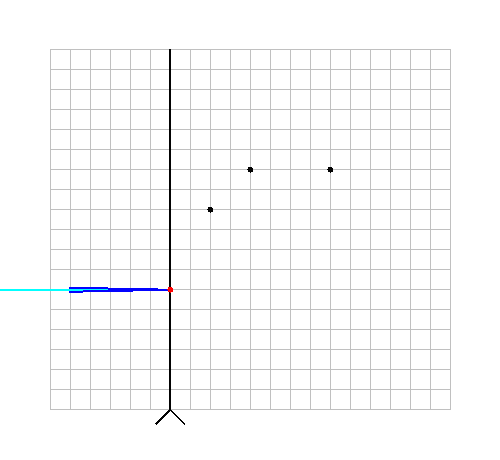
\includegraphics[width=7cm]{capture1}
\end{center}
\caption{Schritt 1}
\label{fig:c1}
\end{figure}

\begin{figure}[h]
\begin{center}
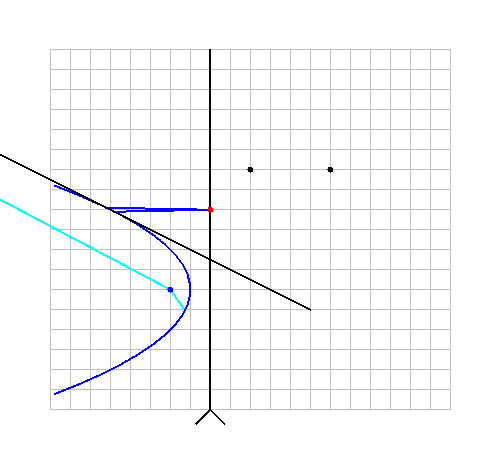
\includegraphics[width=7cm]{capture2}
\end{center}
\caption{Schritt 2}
\label{fig:c2}
\end{figure}

\begin{figure}[h]
\begin{center}
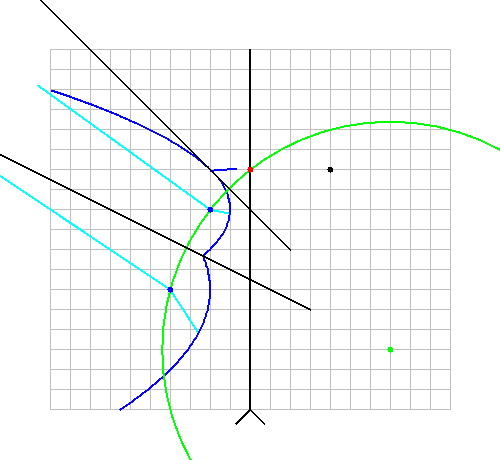
\includegraphics[width=7cm]{capture3}
\end{center}
\caption{Schritt 3}
\label{fig:c3}
\end{figure}

\begin{figure}[h]
\begin{center}
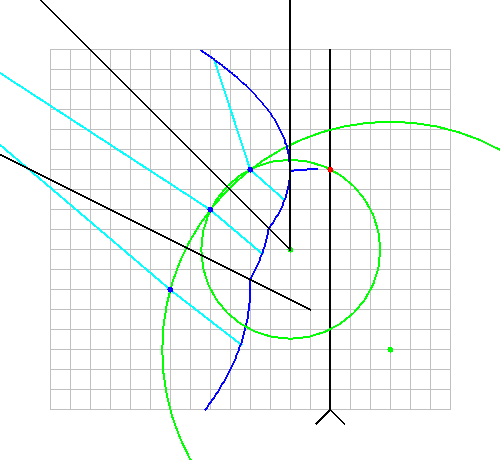
\includegraphics[width=7cm]{capture4}
\end{center}
\caption{Schritt 4}
\label{fig:c4}
\end{figure}

\begin{figure}[h]
\begin{center}
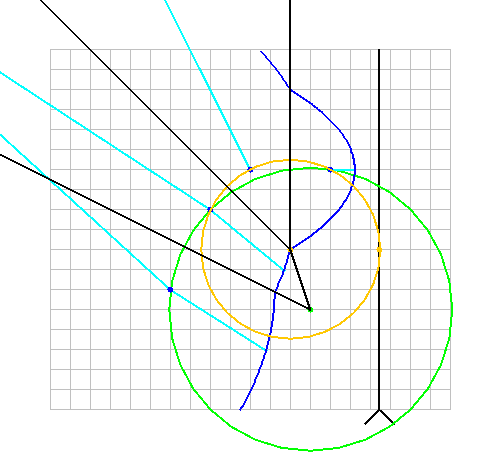
\includegraphics[width=7cm]{capture5}
\end{center}
\caption{Schritt 5}
\label{fig:c5}
\end{figure}

\begin{figure}[h]
\begin{center}
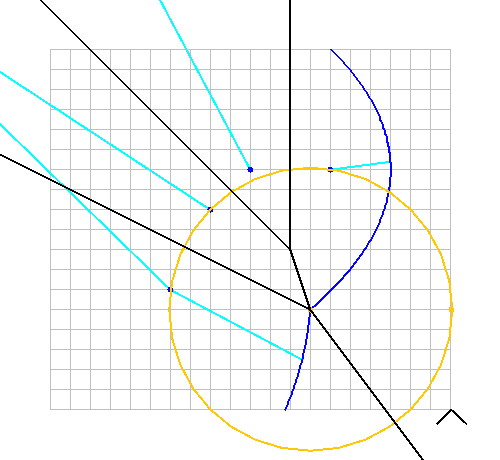
\includegraphics[width=7cm]{capture6}
\end{center}
\caption{Schritt 6}
\label{fig:c6}
\end{figure}

\begin{figure}[h]
\begin{center}
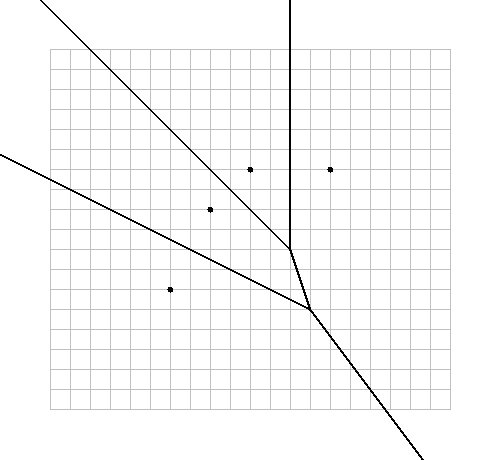
\includegraphics[width=7cm]{capture7}
\end{center}
\caption{Schritt 7}
\label{fig:c7}
\end{figure}